\section{Limite probabilistique des gradients}\label{lim_proba_grad}

Dans la section précédente, nous avons étudié le comportement de la sortie du réseau pour des valeurs élevées de $L$. Cependant, cette analyse ne nous renseigne pas sur le comportement du gradient du coût $p_k = \frac{\partial \mathscr{L}}{\partial h_k} \in \mathbb{R}^d$ durant la rétropropagation, qui est pourtant une donnée cruciale pour évaluer la capacité d'entraînement du réseau à l'initialisation. Par conséquent, cette section se consacrera à l'étude des variations de $\left\| p_0 - p_L \right\| / \left\| p_L \right\|$, toujours dans un contexte où la profondeur du réseau $L$ est grande. Il est important de noter que, en raison de la nature de la rétropropagation, notre attention se porte désormais sur $p_0$ plutôt que sur $p_L$. Nous définissons donc la séquence $(p_k)_{0 \leq k \leq L}$ comme suit :
\begin{align*}
    \qquad & p_k = p_{k+1} + \alpha _L \frac{\partial g(h_k, \theta _{k+1}) ^T}{\partial h}  V_{k+1}^T p_{k+1} \\
    % \Leftrightarrow & \left\| p_k \right\| ^2 = \left\| p_{k+1} \right\| ^2 + \alpha _L ^2 \left\| \frac{\partial g(h_k, \theta _{k+1}) ^T}{\partial h} V_{k+1}^T p_{k+1} \right\| ^2 + 2 \alpha _L \left\langle p_{k+1}, \frac{\partial g(h_k, \theta _{k+1}) ^T}{\partial h}  V_{k+1}^T p_{k+1} \right\rangle 
\end{align*}
Bien que cette récurrence soit similaire à celle des états cachés (\cref{ResNet_equation}), nous ne pouvons pas appliquer les mêmes techniques de preuve utilisées précédement. Cette différence s'explique par la dépendance de $\frac{\partial g(h_k, \theta_{k+1})}{\partial h}$ à $h_k$, et donc à $\theta_1, V_1, \dots, \theta_k, V_k$. Supposer l'indépendance de ces deux quantités serait une hypothèse assez forte, non vérifiée par de nombreuses architectures, comme notre modèle \texttt{res-1}. Ainsi, nous adopterons une autre approche, basée sur la dérivation automatique. Cette méthode nécessite des hypothèses moins contraignantes, mais les résultats obtenus seront exprimés en termes d'espérance plutôt qu'avec une forte probabilité.

Soit $z \in \mathbb{R}^d$. Pour tout $0 \leq i, j \leq L$, définissons $\frac{\partial h_j}{\partial h_i} \in \mathbb{R}^{d \times d}$ comme la matrice Jacobienne de $h_j$ par rapport à $h_i$. Pour rappel, l'élément en position $(m, n)$ de la Jacobienne représente la dérivée de la $m$-ème coordonnée de $h_j$ par rapport à la $n$-ème coordonnée de $h_i$. Soit $q_k(z) = \frac{\partial h_k}{\partial h_0} z$, en appliquant la règle de la chaîne, nous obtenons
\begin{equation}\label{eq:9}
    q_{k+1}(z) = \frac{\partial h_{k+1}}{\partial h_k} q_k(z) = q_k(z) + \alpha _L V_{k+1} \frac{\partial g(h_k, \theta _{k+1})}{\partial h} q_k(z)
\end{equation}
Nous observons une récurrence similaire à celle présentée dans l'\Cref{resnet_equation}. En considérant maintenant que $z$ est une variable aléatoire suivant une distribution gaussienne, il devient possible de décrire la valeur de $\left\| p_0 \right\| / \left\| p_L \right\|$ en fonction du dernier vecteur $q_L(z)$.
\begin{equation}\label{eq:10}
    \frac{\left\| p_0 \right\| ^2}{\left\| p_L \right\| ^2} = \frac{1}{\left\| p_L \right\| ^2} \mathbb{E}_{z \sim \mathcal{N}(0, I_d)}\left(\left| p_0^T z  \right| ^2 \right) = \mathbb{E}_{z \sim \mathcal{N}(0, I_d)}\left(\left| \left(\frac{p_L}{\left\| p_L \right\| } \right)^T q_L(z) \right| ^2 \right)
\end{equation}
avec $ I_d $ la matrice identité sur $ \mathbb{R}^d $. On retrouve la seconde égalité comme conséquence de 
\[
    p_0^T = \left(\frac{\partial \mathscr{L}}{\partial h_0} \right)^T, z = \left(\frac{\partial \mathscr{L}}{\partial h_0} \right)^T \frac{\partial h_L}{\partial h_0} z = p_L^T  q_L(z)
.\]
En résumé, la récurrence énoncée dans l'équation (\ref{eq:9}) va nous permettre de déterminer les bornes de $\left\| q_L(z) \right\|$. Ces résultats pourront ensuite être transposés à $\left\| p_0 \right\| / \left\| p_L \right\|$ en utilisant l'\Cref{eq:10}. Pour ce faire, il nous faudra établir certaines hypothèses sur le rapport $p_L / \left\| p_L \right\|$.

\subsection*{Hypothèses}

\begin{assumption}\label{H3}
    Soit $ b= p_L / \left\| p_L \right\|  $, alors $ \mathbb{E}[b | h_L] = 0 $ et $ \mathbb{E}(b^T b | h_L) = I_d / d $
\end{assumption}
\begin{note}
    Cette hypothèse est facilement vérifiée. Par exemple, en considérant $n_{out} = 1$ et en utilisant l'entropie croisée pour une classification binaire, ou bien l'erreur quadratique dans le cadre d'une régression.
\end{note}

L'hypothèse suivante est l'équivalent pour les gradients de ce qui est énoncé dans \Cref{H2}.
\begin{assumption}\label{H4}
    On a, presque surement, 
    \[
        \frac{\left\| q_k \right\| ^2}{2} \leq \mathbb{E}\left(\left\| \frac{\partial g(h_k, \theta _{k+1})}{\partial h} q_k  \right\| ^2 | h_k, q_k \right) \leq \left\| q_k \right\| ^2
    .\]
\end{assumption}

L'\Cref{H4} s'applique à toutes les architectures répertoriées dans la \Cref{tab:resnet_architectures}, comme le démontre la proposition suivante.
\begin{proposition}\label{prop5}
    Soit les réseaux \texttt{res-1}, \texttt{res-2} et \texttt{res-3} définit dans la \Cref{tab:resnet_architectures}. Supposons l'\Cref{H1} satisfaite et $ \sigma  $ dérivable presque partout avec $ a \leq \sigma ^\prime \leq b $. Alors
    \begin{itemize}
        \item [(i)] L'\Cref{H4} est valide pour \texttt{res-1}
        \item [(ii)] L'\Cref{H4} est valide pour \texttt{res-2} et \texttt{res-3} dès lors que les entrées de $ \sqrt{d} W_{k+1}, 0 \leq k \leq L-1 $ sont des variables aléatoires de variance unitaire, i.i.d, symétriques et indépendante de $ d $ et $ L $.
    \end{itemize}
\end{proposition}

Les propositions \Cref{prop6} et \ref{prop7} sont les homologues des \Cref{prop2} et \ref{prop3} pour l'analyse du gradient du coût à l'initialisation.

\begin{proposition}\label{prop6}
    Soit un ResNet (\ref{tab:resnet_architectures}) tel que les \Cref{H1} à \ref{H4} sont satisfaites. Si $ L \alpha _L ^2 \leq 1 $ alors, pour tout $ \delta \in (0,1) $ avec une probabilité d'au moins $ 1 - \delta  $ 
    \[
        \frac{\left\| p_0 - p_L \right\| ^2 }{\left\| p_l \right\| ^2 } \leq \frac{2 L \alpha _L ^2}{\delta }
    .\]
\end{proposition}

\begin{proposition}\label{prop7}
    Soit un ResNet (\ref{tab:resnet_architectures}) tel que les \Cref{H1} à \ref{H4} sont satisfaites. Alors 
    \[
        (1 + \frac{1}{2} \alpha _L ^2)^L - 1 \leq \mathbb{E}\left( \frac{\left\| p_0 - p_L \right\| ^2 }{\left\| p_l \right\| ^2 } \right) \leq (1 + \alpha _L ^2)^L - 1
    .\]
\end{proposition}

De façon similaire au \Cref{cor4}, le \Cref{cor8} est déduit à partir des \Cref{prop6} et \ref{prop7}.

\begin{cor}\label{cor8}
    Soit un ResNet (\ref{tab:resnet_architectures}) tel que les Hypothèses 1 à 4 sont satisfaites. En posant $ \alpha _L = 1 / L^\beta $ avec $ B > 0 $, on obtient 
    \begin{enumerate}
        \item [(i)] Si $ \beta > 1/2 $, alors 
        \[
            \frac{\left\| p_0 - p_L \right\| }{\left\| p_l \right\|  } \xrightarrow[L \to \infty]{\mathbb{P}} 0
        .\]
        \item [(ii)] Si $ \beta < 1/2 $ alors 
        \[
            \mathbb{E}\left(\frac{\left\| p_0 - p_L \right\| ^2 }{\left\| p_l \right\| ^2 }\right) \xrightarrow[L \to \infty]{\mathbb{P}} \infty
        .\]
        \item [(iii)] Si $ \beta = 1/2 $ alors
        \[
            \exp (\frac{1}{2}) - 1 \leq \mathbb{E}\left(\frac{\left\| p_0 - p_L \right\| ^2 }{\left\| p_l \right\| ^2 }\right) \leq \exp (4) - 1
        .\]
    \end{enumerate}
    Ce corrolaire est illustré dans la \Cref{fig:cor8}.\todo{export la figure du pdf avec Windows}
\end{cor}

\begin{figure}[H]
    \centering
    % 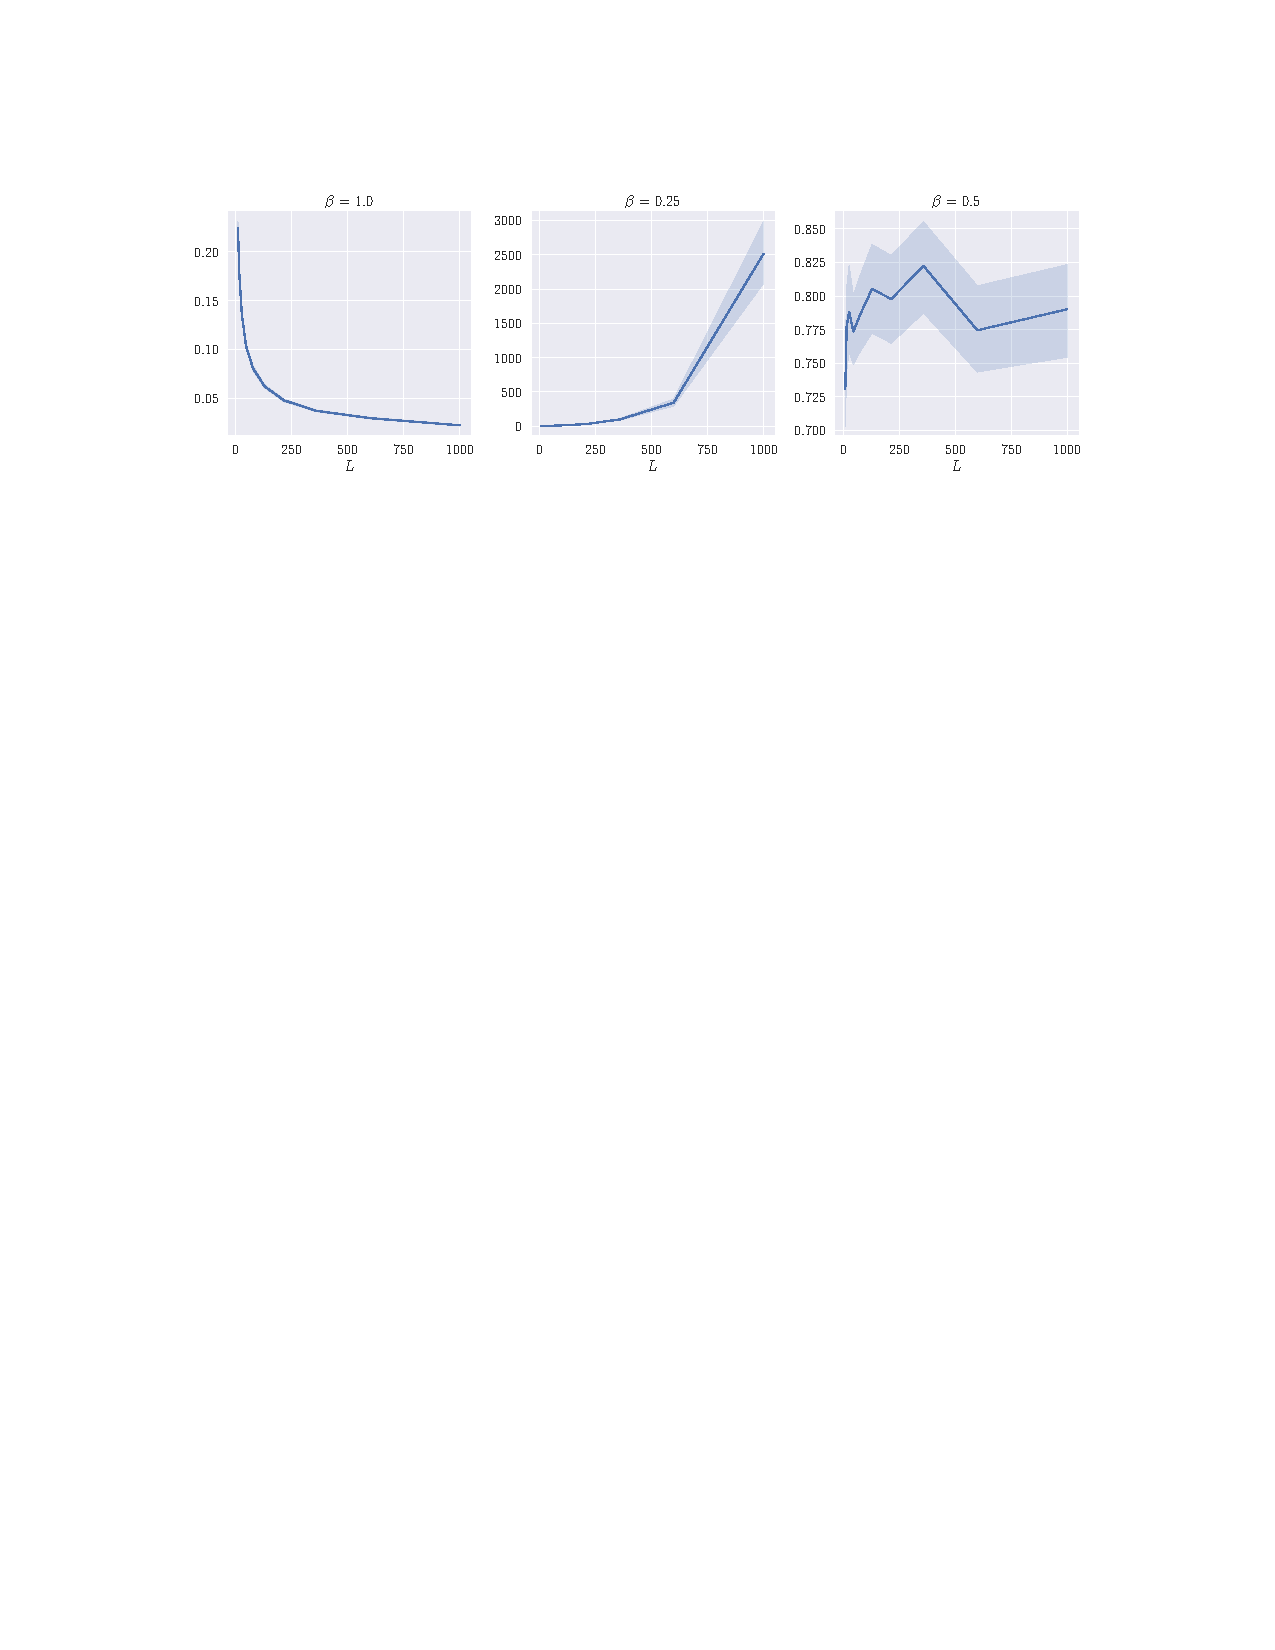
\includegraphics[width=.95\textwidth]{figs/figure_cor8.pdf}
    \caption{Illustration du corollaire \ref{cor8}. Évolution de $ \left\| p_0 - p_L \right\| / \left\| p_L \right\| $ en fonction de $ L $ pour différente valeur de $ \beta  $.}
    \label{fig:cor8}
\end{figure}

\section{Conclusion}
Dans ce chapitre, nous avons examiné comment le comportement des gradients et des états cachés est influencé par la valeur de $\beta$, qui se décline en trois cas distincts :
\begin{itemize}
    \item $\beta < 1/2$ : Une explosion qui empêche l'entraînement du réseau.
    \item $\beta > 1/2$ : Un effet d'identité qui diminue les performances du réseau.
    \item $\beta = 1/2$ : Une limite non-dégénérée favorable.
\end{itemize}
Il est intéressant de noter que la valeur $\beta = 1/2$ joue un rôle clé. De manière surprenante, cette valeur trouve une interprétation spécifique dans l'étude des ResNet dans un cadre continu, sujet que nous aborderons dans le chapitre suivant.
